\chapter{Contact Parameters Tuning}

As explained in \cref{sec:back_contacts}, the choice of the integrator, the integration step size, and the contact parameters can have a significant impact on the simulation results. In this section, we present the results of the contact parameters tuning process, which has been the backbone of the simulations in \jaxsim.
In order to have a better understanding of the contact model, multiple tests have been performed using the same model trained in the \ac{RL} framework. This section presents the results of these tests and the conclusions drawn from them.

For what regards the choice of ground stiffness and damping coefficient, if we recall the theory presented in the matter of smooth contacts in \cref{sec:back_contacts}, the choice has been made by considering the overall mass of the robot and by imposing a static penetration depth of $1$ millimeter.

\begin{equation}
    M\ddot{s} + D\dot{s} + Ks - Mg = \sum _i F _i = 0 \rightarrow s _{static} = \frac{Mg}{K} < 0.001 \text{m}
\end{equation}

where $s$ is the penetration depth, $g$ is the gravity acceleration, $M$ is the mass, $D$ is the damping coefficient, $K$ is the stiffness coefficient.
If we force a critical damping condition, we can compute the damping coefficient as:

\begin{equation}
    \zeta = \frac{D}{2\sqrt{MK}} \rightarrow D = 2\sqrt{MK}\zeta
\end{equation}

we get to a damping coefficient of $c_{crit} = 0.2$ Ns/m. The ground stiffness has been chosen to be $k = 1000$ N/m, which is a reasonable value for a concrete floor.

For the choice of integrators and integration step size, multiple tests have been performed. Two main integrators available in \jaxsim have been tested: \textit{semi-implicit Euler}, which consists of a first-order integrator, and \textit{Runge-Kutta 4}, which is a fourth-order integrator. The integration step size has been varied between $5$ and $0.5$ milliseconds. The contact parameters have been kept constant during the simulations.

\begin{figure}
    \centering
    \caption{Runge-Kutta 4 Integration with different Step Sizes.}
    \label{fig:rk4}
    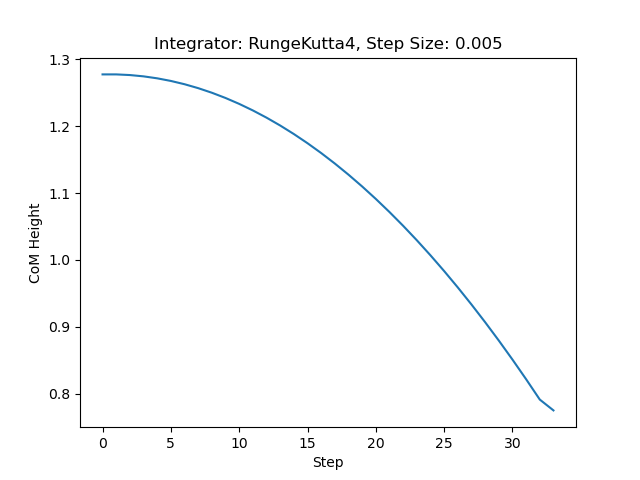
\includegraphics[width=0.45\textwidth]{Images/rk4_5ms.png}
    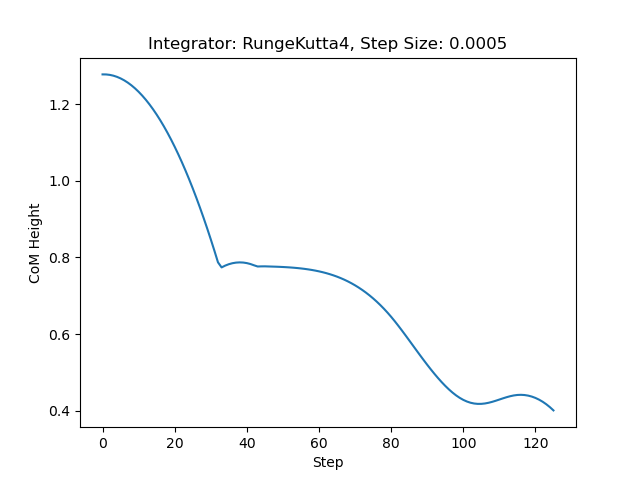
\includegraphics[width=0.45\textwidth]{Images/rk4_05ms.png}
\end{figure}

As can be noticed from \cref{fig:rk4}, the Runge-Kutta 4 integrator is stable only for the smallest step size, which is $0.5$ milliseconds. For the largest step size, the integrator is not stable and the simulation stopped after only $30$ seconds as it started to produce \textit{Not-a-Number} (NaN) values.

\begin{figure}
    \centering
    \caption{Semi-Implicit Euler Integration with different Step Sizes.}
    \label{fig:sie}
    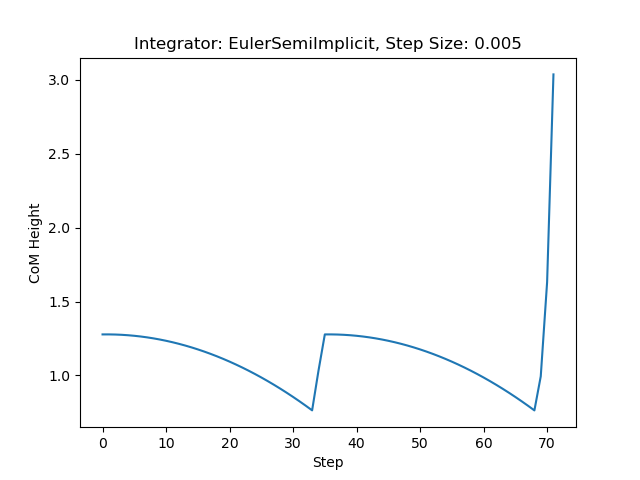
\includegraphics[width=0.45\textwidth]{Images/sie_5ms.png}
    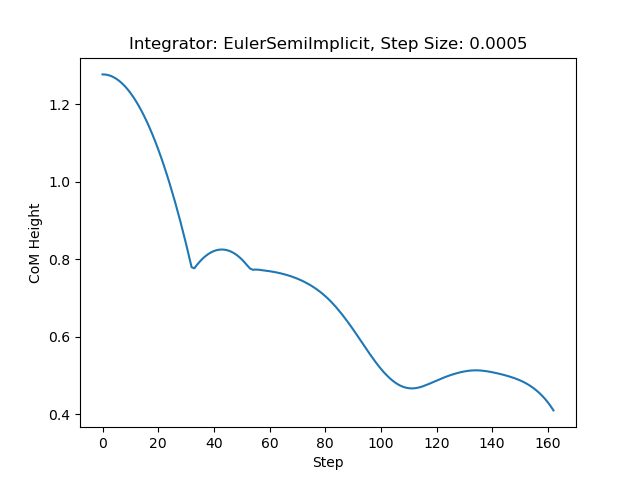
\includegraphics[width=0.45\textwidth]{Images/sie_05ms.png}
\end{figure}

The \textit{semi-implicit Euler} integrator is also not stable for the largest step size, yet being much faster for computation with respect to the Runge-Kutta 4 integrator, it has been chosen as the integrator for the simulations. In fact RK4 involves computing the full robot dynamics four times, drastically increasing the overall computation time.

The integration step size has been chosen to be $0.5\text{m}s$ as it represented a good tradeoff between integration stability and computational effort.
